\documentclass[a4paper,11pt]{report}

\usepackage{amsmath}
\usepackage{fullpage}
\usepackage{bussproofs}
\usepackage{mathpartir}
\usepackage{url}
\usepackage{placeins}

\usepackage{prooftrees}
\newcommand*{\equal}{=}
\newcommand*{\disj}{,}

\usepackage[cache=false]{minted}

\author{Sylvain Julmy}
\date{\today}

\setlength{\parindent}{0pt}

\newminted{prolog}{frame=single, framesep=6pt,
  breaklines=true,fontsize=\scriptsize,linenos}
\newmintedfile{prolog}{frame=single, framesep=6pt,
  breaklines=true,fontsize=\scriptsize}
\newmintinline{prolog}{}
\newcommand{\ex}[3]{\prologfile[firstline=#1,lastline=#2]{#3.pl}}

\begin{document}

\begin{center}
  \Large{
    Functional and Logic Programming\
    Fall 2017
  }
  
  \noindent\makebox[\linewidth]{\rule{\linewidth}{0.4pt}}
  S12 : Prolog
  \noindent\makebox[\linewidth]{\rule{\linewidth}{0.4pt}}

  \begin{flushleft}
    Professor : Le Peutrec Stephane
    
    Assistant : Lauper Jonathan
  \end{flushleft}

  \noindent\makebox[\linewidth]{\rule{\textwidth}{1pt}}
\end{center}
\section*{Exercise 1}

\subsection*{\texttt{myMap}}
\ex{10}{16}{ex1}

\subsection*{\texttt{myPartition}}
\ex{19}{28}{ex1}

\subsection*{\texttt{filter}}
\ex{31}{39}{ex1}

\subsection*{\texttt{filterWithFindall}}
\ex{42}{45}{ex1}

\subsection*{\texttt{myIntersection}}
\ex{48}{50}{ex1}

\subsection*{Some utility predicats}
\ex{52}{67}{ex1}

\newpage

\section*{Exercise 2}

\ex{9}{73}{ex2_bis}

\newpage

\section*{Exercise 3}

We would use the following ebnf grammar for our ``grammar'' syntax :

\begin{verbatim}
grammar ::= rule grammar | rule
rule ::= rule_name "->" rule_body
rule_body ::= rule_body_part_rec "|" rule_body | rule_body_part_rec
rule_body_part_rec ::= rule_body_part rule_body_part_rec | rule_body_part
rule_body_part ::= rule_name | atomName

rule_name ::= "r_" anyChar*
atomName ::= (lowerCase - "r") (anyChar - "_") lowerCase* | lowerCase anyChar*

lowerCase ::= "a" | "b" | "c" | "d" | "e" | "f" | "g"
            | "h" | "i" | "j" | "k" | "l" | "m" | "n"
            | "o" | "p" | "q" | "r" | "s" | "t" | "u"
            | "v" | "w" | "x" | "y" | "z"

anyChar ::= #x9 | #xA | #xD | [#x20-#xD7FF] | [#xE000-#xFFFD] | [#x10000-#x10FFFF]
\end{verbatim}

Note :
\begin{itemize}
\item The \verb|anyChar| rule correspond any Unicode character, excluding the
  surrogate blocks, FFFE, and FFFF. It as been taken from
  \url{https://www.w3.org/TR/xml/#NT-Char}.
\item We use the Extended Backus-Naur Form (EBNF) to specify the syntax.
\item The syntacic diagram are available from figure \ref{fig:grammar} to
  \ref{fig:rule_name}.
\item We don't show the diagram for the \verb|rule_name|, \verb|atomName| or \verb|lowerCase|.
\end{itemize}

\begin{figure}[ht]
  \centering
  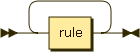
\includegraphics[width=0.2\textwidth]{figures/grammar}
  \caption{ENBF diagram for the rule ``grammar''}
  \label{fig:grammar}
\end{figure}

\begin{figure}[ht]
  \centering
  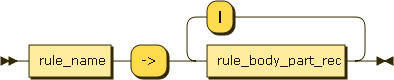
\includegraphics[width=0.5\textwidth]{figures/rule}
  \caption{ENBF diagram for the rule ``rule''}
  \label{fig:rule}
\end{figure}

\begin{figure}[ht]
  \centering
  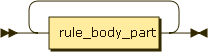
\includegraphics[width=0.35\textwidth]{figures/rule_body_part_rec}
  \caption{ENBF diagram for the rule ``rule\_body\_part\_rec''}
  \label{fig:rule_body_part_rec}
\end{figure}

\begin{figure}[ht]
  \centering
  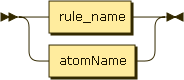
\includegraphics[width=0.3\textwidth]{figures/rule_body_part}
  \caption{ENBF diagram for the rule ``rule\_body\_part''}
  \label{fig:rule_body_part}
\end{figure}

\begin{figure}[ht]
  \centering
  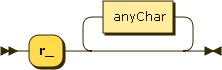
\includegraphics[width=0.4\textwidth]{figures/rule_name}
  \caption{ENBF diagram for the rule ``rule\_name''}
  \label{fig:rule_name}
\end{figure}

\FloatBarrier

\subsection*{Implementation}
\ex{11}{62}{ex3}

\end{document}

%%% Local Variables:
%%% TeX-command-extra-options: "-shell-escape"
%%% mode: latex
%%% End:
Extended Backus-Naur Form
